%! Author = Len Washington III
%! Date = 9/12/2023

% Preamble
\documentclass[8]{cs430lecture}

% Packages

% Document
\begin{document}

%<*Lecture-Activity-8>
\maketitle
\openingquestions
\begin{itemize}
	\item If we have 17 distinct items to sort, what is the height of the decision tree that represents all possible orderings of the 17 items? \answer{The height of the decision tree is $\lceil \log_{2}(17!) \rceil = \lceil 48.337603311133 \rceil = 49$ and the possible orderings of the 17 items is $17!$. However, $\log_{2}(n!) = \theta(n\lg n)$.}
\end{itemize}

\section{Comparison Sorts}\label{sec:comparison-sorts}
The sorted order they determine is based only on comparisons between the input elements. That is, given two elements $a_{i}$ and $a_{j}$, we perform one of the tests $a_{i} < a_{j}$, $a_{i} = a_{j}$, or $a_{i} > a_{j}$ to determine their relative order.\\

\noindent Claim: We must make at least $\Omega(n\lg n)$ comparisons in the general case.\\

\noindent The decision-tree model
\begin{itemize}
	\item Abstraction of any comparison sort.
	\item Represents comparisons made by a specific sorting algorithm on inputs of a given size.
	\item Abstracts away everything else: control and data movement
	\item View the tree as if the algorithm splits in two at each node, based on the information it has determined up to that point; The tree models all possible execution traces.\\
\end{itemize}

\noindent Each internal node is labeled by indices of array elements \textbf{from their original positions}. Each leaf is labeled by the permutation of orders that the algorithm determines.

\begin{enumerate}[label=\arabic*.]
    \item How many possible permutations of $n$ items are there (at least one of them must be sorted)? In the decision tree model, how many leaves are there for $n$ items? For a binary tree to have that many leaves, how many levels does it need? Why do we care about how many levels are in the decision tree? \answer{There are n! possible permutations. A binary tree would have $2^{\mbox{height}}$ levels.}
\end{enumerate}

\section{Linear Time Sorting -- Counting Sort}\label{sec:linear-time-sorting-counting-sort}
If we do not use comparison of keys to sort data, how can we sort data? It seems comparing items is necessary for sorting.
\begin{itemize}
	\item Counting sort assumes that each of the $n$ input elements is an integer in the range $0$ to $k$, for some integer $k$. When $k=O(n)$, the sort runs in $T(n)$ time (best if the size of the range is $k \lll n$)
	\item For each input element $x$, count how many elements are equal to $x$ then use this to count how many elements are $\leq x$. This information can be used to place element $x$ directly into its position in the output array.
	\item Does not sort in place, needs $2^{\mbox{nd}}$ array size $n$ and $3^{\mbox{rd}}$ array size $k$
\end{itemize}

\begin{figure}[H]
	\centering
	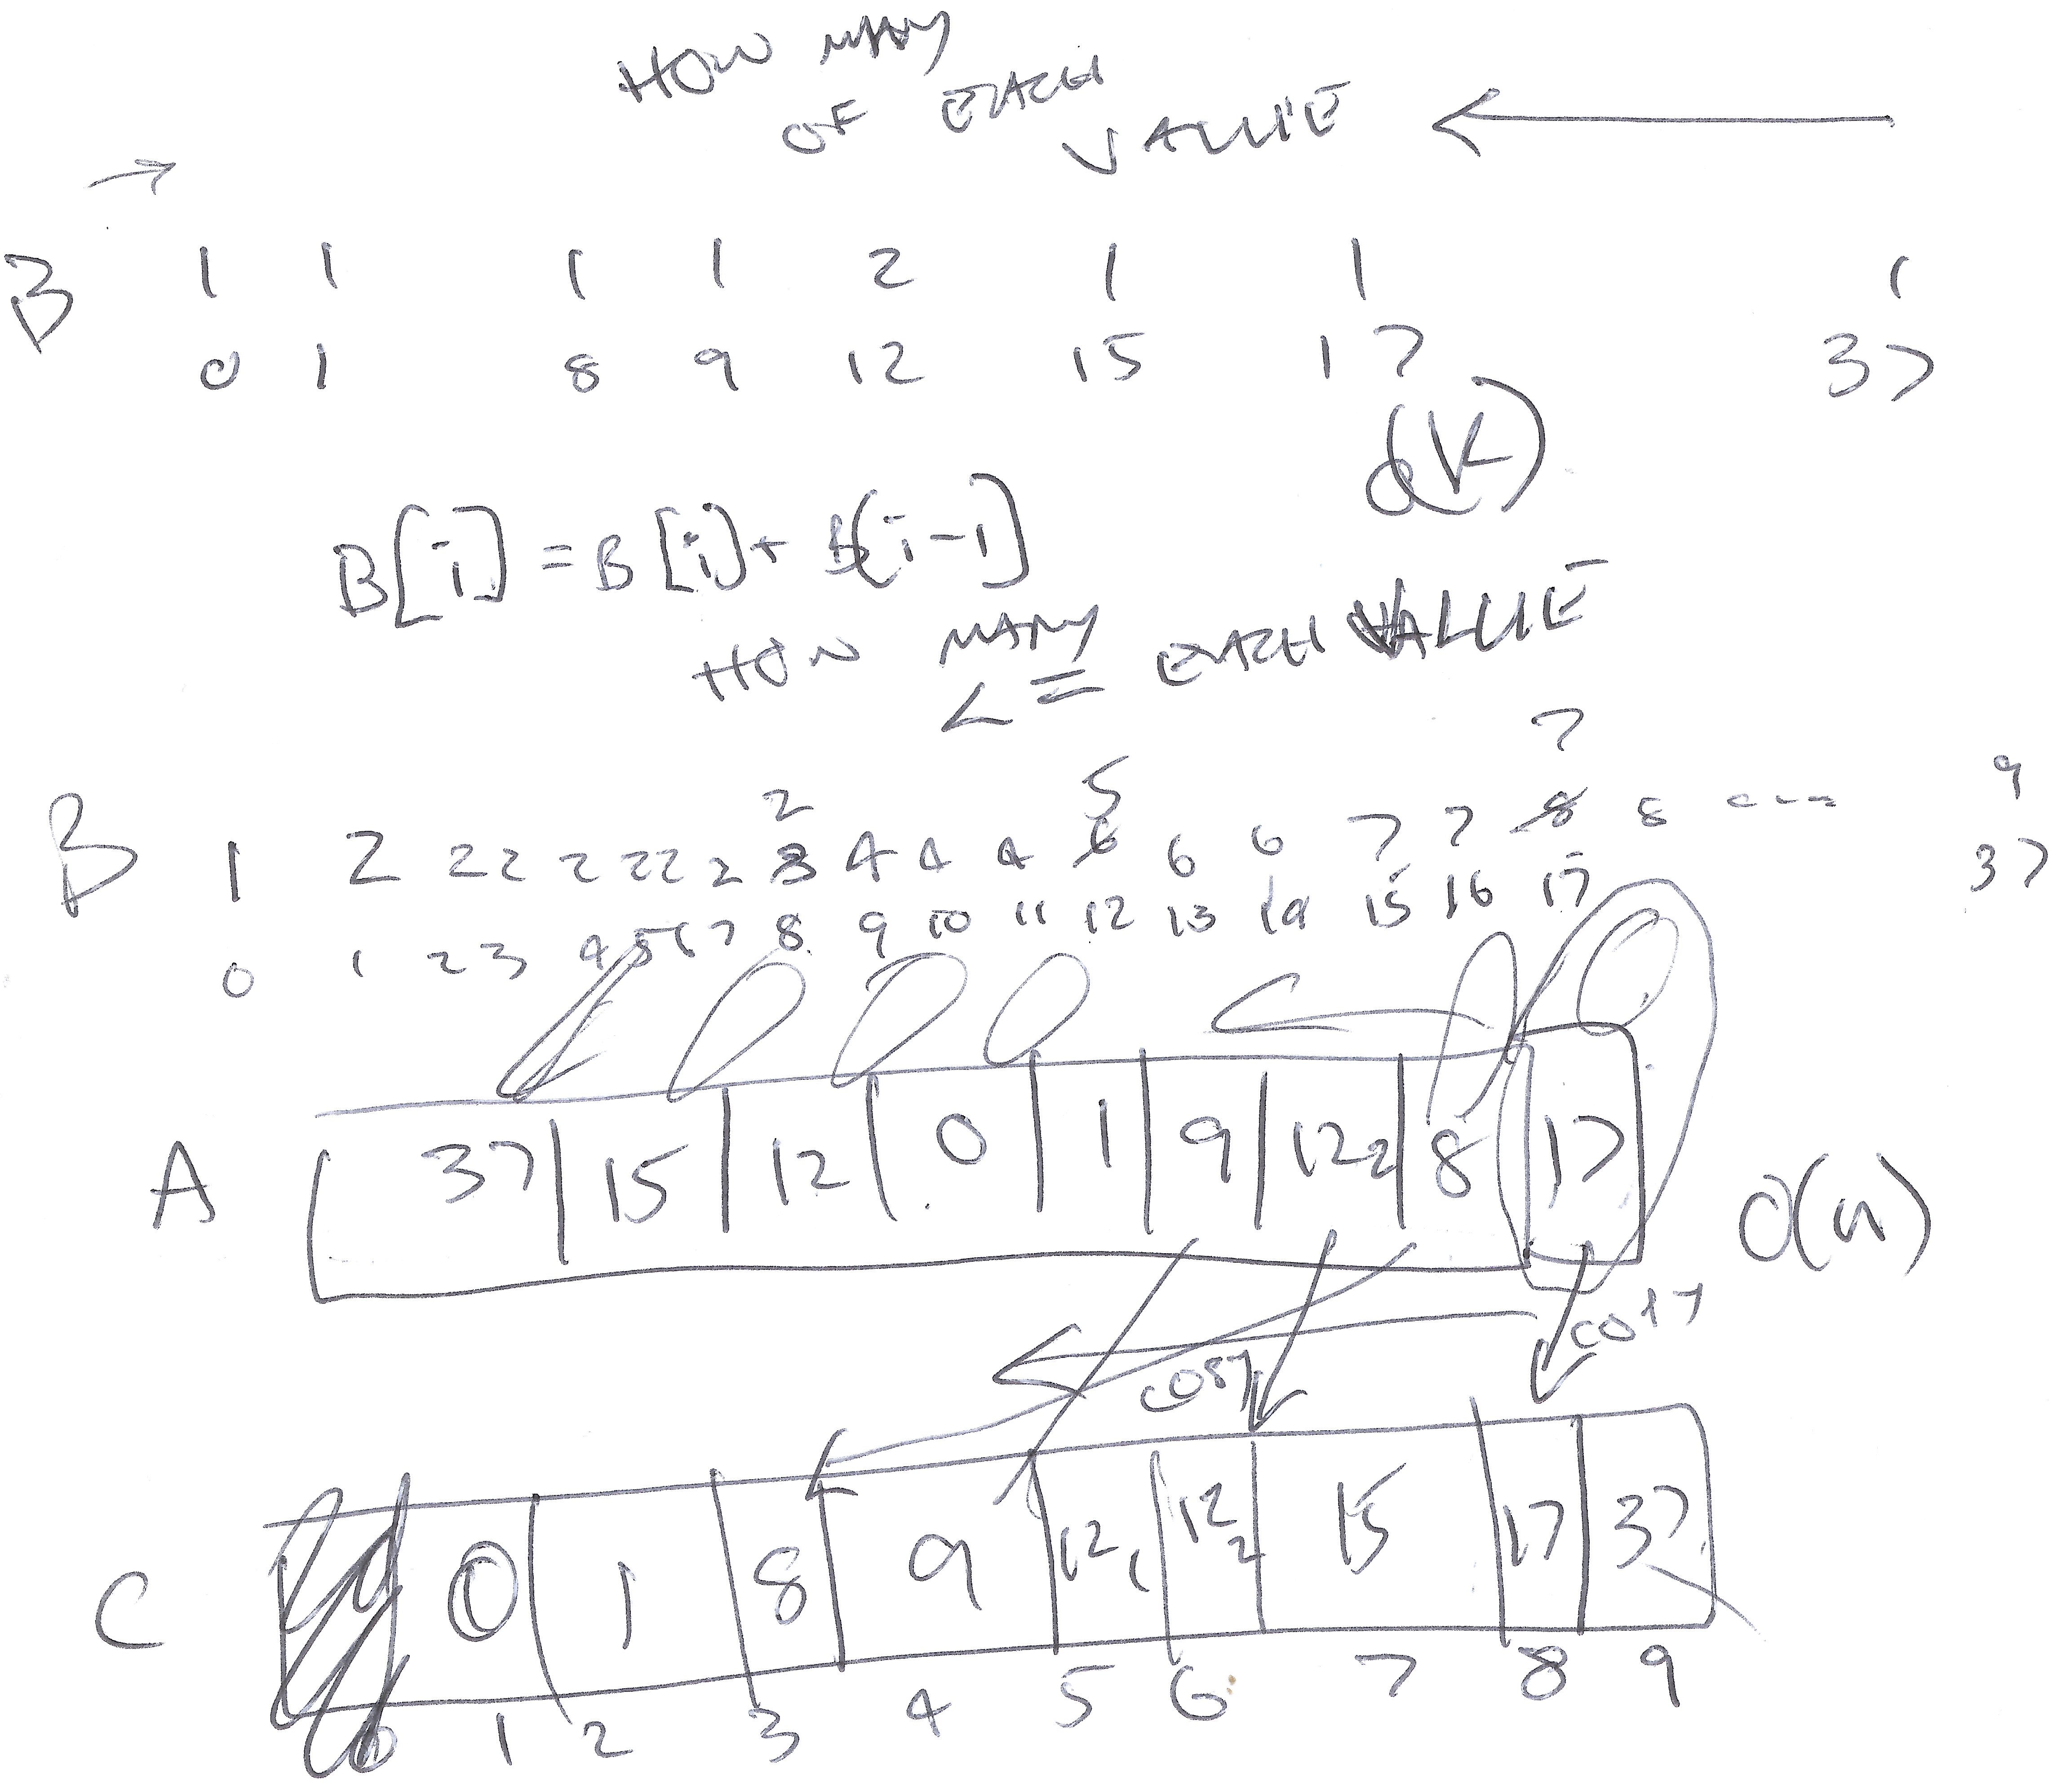
\includegraphics[width=\textwidth]{counting_sort_demo}
	\caption{Counting sort demonstration.}
	\label{fig:counting-sort-demo}
\end{figure}


\begin{enumerate}[label=\arabic*., start=2]
    \item Write pseudocode for counting sort. \answer{\begin{algorithm}[H]
    	\caption{Counting Sort}\label{alg:counting-sort}
    	\begin{algorithmic}[1]
    	\Function{CountingSort}{$A$}\Comment{$A$=original array, $B$=size-$k$ counters, $C$=size-$n$ sorted data}
			\For{$i=1\dots n$}
				\State $B$[$A$[$i$]]++					\Comment{counters}
			\EndFor
			\For{$j=1\dots k$}
				\State $B$[$j$] = $B$[$j$] + $B$[$j-1$]	\Comment{$\leq$ counters}
			\EndFor
			\For{$i=n\dots 1$}
				\State $C$[$B$[$A$[i]]] = $A$[i]
				\State $B$[$A$[i]]{-}{-}
			\EndFor
    	\EndFunction
    	\end{algorithmic}
    \end{algorithm}}
	\item Demo counting sort on this data:\begin{table}[H]
	    \centering
	    \begin{threeparttable}
			\label{tab:counting-demo}
			\begin{tabular}{|c|c|c|c|c|c|c|c|}
				\toprule
				2 & 5 & 3 & 0 & 2 & 3 & 0 & 3\\
				\bottomrule
			\end{tabular}
		\end{threeparttable}
	\end{table}
\end{enumerate}

\noindent Counting sort is best on large amounts of data where the range of the data is small. Like many single digit numbers. However, we can use counting sort multiple times to sort multiple digit numbers, starting with the right most digit, etc. This is called Radix Sort.

\begin{table}[H]
    \centering
    \begin{threeparttable}
		\caption{Radix Sort}
		\label{tab:radix-sort}
		\begin{tabular}{ccccccc}
			\toprule
			329 & 					& 72\colorbox{lightgray}{0} & 					& 7\colorbox{lightgray}{2}0 & 				& \colorbox{lightgray}{3}29\\
			457 & 					& 35\colorbox{lightgray}{5} & 					& 3\colorbox{lightgray}{2}9 & 				& \colorbox{lightgray}{3}55\\
			657 & 					& 43\colorbox{lightgray}{6} & 					& 4\colorbox{lightgray}{3}6 & 				& \colorbox{lightgray}{4}36\\
			839 & $\rightarrow$ 	& 45\colorbox{lightgray}{7} & $\rightarrow$ 	& 8\colorbox{lightgray}{3}9 & $\rightarrow$	& \colorbox{lightgray}{4}57\\
			436 & 					& 65\colorbox{lightgray}{7} & 					& 3\colorbox{lightgray}{5}5 & 				& \colorbox{lightgray}{6}57\\
			720 & 					& 32\colorbox{lightgray}{9} & 					& 4\colorbox{lightgray}{5}7 & 				& \colorbox{lightgray}{7}20\\
			355 & 					& 83\colorbox{lightgray}{9} & 					& 6\colorbox{lightgray}{5}7 & 				& \colorbox{lightgray}{8}39\\
			\bottomrule
		\end{tabular}
		\begin{tablenotes}
			\small
			\item \answer{Each $O(k)$ where $k$ is $0\rightarrow 9$. This makes the overall $O=O(n + \mbox{digits}*k)=O(n + 10k)$, but k is insignificant to $n$, so it's essentially $O(n)$.}
		\end{tablenotes}
	\end{threeparttable}
\end{table}

\noindent An important property of counting sort is that it is \textbf{\emph{stable}}: numbers with the same value appear in the output array in the same order as they do in the input array. That is, it breaks ties between two numbers by the rule that whichever number appears first in the input array appears first in the output array. Normally, the property of stability is important only when satellite data are carried around with the element being sorted. Counting sort's ability is important for another reason: counting sort is often used as a subroutine in radix sort. As we shall see in the next section, in order for radix sort to work correctly, counting sort must be stable.

\begin{enumerate}[label=\arabic*., start=4]
    \item Which of these sorts can be stable:
	\begin{itemize}
		\item \answer{Insertion Sort}
		\item \textcolor{red}{Selection Sort} $\leftarrow$ \answer{you could potentially jump an item passed its duplicate}
		\item \answer{Bubble Sort}
		\item {Merge Sort} $\leftarrow$ \answer{depends on the merge}
		\item \textcolor{red}{Quick Sort} $\leftarrow$ \answer{the paritioning might not be stable and an item can be jumped passed its duplicate.}
		\item \textcolor{red}{Heap Sort}
	\end{itemize}
\end{enumerate}
%</Lecture-Activity-8>

\end{document}